\documentclass[]{article}
\usepackage{lmodern}
\usepackage{amssymb,amsmath}
\usepackage{ifxetex,ifluatex}
\usepackage{fixltx2e} % provides \textsubscript
\ifnum 0\ifxetex 1\fi\ifluatex 1\fi=0 % if pdftex
  \usepackage[T1]{fontenc}
  \usepackage[utf8]{inputenc}
\else % if luatex or xelatex
  \ifxetex
    \usepackage{mathspec}
  \else
    \usepackage{fontspec}
  \fi
  \defaultfontfeatures{Ligatures=TeX,Scale=MatchLowercase}
\fi
% use upquote if available, for straight quotes in verbatim environments
\IfFileExists{upquote.sty}{\usepackage{upquote}}{}
% use microtype if available
\IfFileExists{microtype.sty}{%
\usepackage{microtype}
\UseMicrotypeSet[protrusion]{basicmath} % disable protrusion for tt fonts
}{}
\usepackage{hyperref}
\PassOptionsToPackage{usenames,dvipsnames}{color} % color is loaded by hyperref
\hypersetup{unicode=true,
            pdftitle={CS 229 Homework},
            pdfauthor={Tyler Neylon},
            colorlinks=true,
            linkcolor=black,
            citecolor=Blue,
            urlcolor=Blue,
            breaklinks=true}
\urlstyle{same}  % don't use monospace font for urls
\usepackage{graphicx,grffile}
\makeatletter
\def\maxwidth{\ifdim\Gin@nat@width>\linewidth\linewidth\else\Gin@nat@width\fi}
\def\maxheight{\ifdim\Gin@nat@height>\textheight\textheight\else\Gin@nat@height\fi}
\makeatother
% Scale images if necessary, so that they will not overflow the page
% margins by default, and it is still possible to overwrite the defaults
% using explicit options in \includegraphics[width, height, ...]{}
\setkeys{Gin}{width=\maxwidth,height=\maxheight,keepaspectratio}
\IfFileExists{parskip.sty}{%
\usepackage{parskip}
}{% else
\setlength{\parindent}{0pt}
\setlength{\parskip}{6pt plus 2pt minus 1pt}
}
\setlength{\emergencystretch}{3em}  % prevent overfull lines
\providecommand{\tightlist}{%
  \setlength{\itemsep}{0pt}\setlength{\parskip}{0pt}}
\setcounter{secnumdepth}{5}
% Redefines (sub)paragraphs to behave more like sections
\ifx\paragraph\undefined\else
\let\oldparagraph\paragraph
\renewcommand{\paragraph}[1]{\oldparagraph{#1}\mbox{}}
\fi
\ifx\subparagraph\undefined\else
\let\oldsubparagraph\subparagraph
\renewcommand{\subparagraph}[1]{\oldsubparagraph{#1}\mbox{}}
\fi
\usepackage{subfig}
\AtBeginDocument{%
\renewcommand*\figurename{Figure}
\renewcommand*\tablename{Table}
}
\AtBeginDocument{%
\renewcommand*\listfigurename{List of Figures}
\renewcommand*\listtablename{List of Tables}
}
\usepackage{float}
\floatstyle{ruled}
\makeatletter
\@ifundefined{c@chapter}{\newfloat{codelisting}{h}{lop}}{\newfloat{codelisting}{h}{lop}[chapter]}
\makeatother
\floatname{codelisting}{Listing}
\newcommand*\listoflistings{\listof{codelisting}{List of Listings}}

\title{CS 229 Homework}
\author{Tyler Neylon}
\date{345.2016}

% Begin custom, non-pandoc commands.

\newcommand{\latexonlyrule}{\rule}

% End custom, non-pandoc commands.

\begin{document}
\maketitle

\newcommand{\R}{\mathbb{R}}
\newcommand{\eqnset}[1]{\left.\mbox{$#1$}\quad\quad\right\rbrace}
\newcommand{\tr}{\text{tr}\;}
\renewcommand{\th}{\theta}
\newcommand{\toi}{^{(i)}}

These are solutions to the most recent problems posted for Stanford's CS
229 course, as of June 2016. I'm not sure if this course re-uses old
problems, but please don't copy the answers if so. This document is also
available as a
\href{http://tylerneylon.com/notes/cs229/cs229hw.pdf}{pdf}.

\section{Problem set 1}\label{problem-set-1}

\subsection{Logistic regression}\label{logistic-regression}

\subsubsection{Part (a)}\label{part-a}

The problem is to compute the Hessian matrix \(H\) for the function

\[J(\th) = -\frac{1}{m}\sum_{i=1}^m\log(g(y\toi x\toi)),\]

where \(g(z)\) is the logistic function, and to show that \(H\) is
positive semi-definite; specifically, that \(z^THz\ge 0\) for any vector
\(z.\)

We'll use the fact that \(g'(z) = g(z)(1-g(z)).\) We'll also note that
since all relevant operations are linear, it will suffice to ignore the
summation over \(i\) in the definition of \(J.\) I'll use the notation
\(\partial_j\) for \(\frac{\partial}{\partial\th_j},\) and introduce
\(t\) for \(y\th^Tx.\) Then

\[-\partial_j(mJ) = \frac{g(t)(1-g(t))}{g(t)}x_jy = x_jy(1-g(t)).\]

Next

\[-\partial_k\partial_j(mJ) = x_jy\big(-g(t)(1-g(t))\big)x_ky,\]

so that

\[\partial_{jk}(mJ) = x_jx_ky^2\alpha,\]

where \(\alpha = g(t)(1-g(t)) > 0.\)

Thus we can use repeated-index summation notation to arrive at

\[z^THz = z_ih_{ij}z_j = (\alpha y^2)(z_ix_ix_jz_j)
        = (\alpha y^2)(x^Tz)^2 \ge 0.\]

This completes this part of the problem.

\subsubsection{Part (b)}\label{part-b}

Here is a matlab script to solve this part of the problem:

\begin{verbatim}
% problem1_1b.m
%
% Run Newton's method on a given cost function for a logistic
% regression setup.
%

printf('Running problem1_1b.m\n');

% Be able to compute J.
function val = J(Z, theta)
  [m, _] = size(Z);
  g      = 1 ./ (1 + exp(Z * theta));
  val    = -sum(log(g)) / m;
end

% Setup.
X      = load('logistic_x.txt');
[m, n] = size(X);
X      = [ones(m, 1) X];
Y      = load('logistic_y.txt');
Z      = diag(Y) * X;

% Initialize the parameters to learn.
old_theta =  ones(n + 1, 1);
theta     = zeros(n + 1, 1);
i         = 1;  % i = iteration number.

% Perform Newton's method.
while norm(old_theta - theta) > 1e-5
  printf('J = %g\n', J(Z, theta));
  printf('theta:\n');
  disp(theta);
  printf('Running iteration %d\n', i);

  g         = 1 ./ (1 + exp(Z * theta));
  f         = (1 - g);
  alpha     = f .* g;
  A         = diag(alpha);
  H         = Z' * A * Z / m;
  nabla     = Z' * f / m;
  old_theta = theta;
  theta     = theta - inv(H) *  nabla;

  i++;
end

% Show and save output.
printf('Final theta:\n');
disp(theta);
save('theta.mat', 'theta');
\end{verbatim}

Because I have copious free time, I also wrote a Python version. Also
because I'm learning numpy and would prefer to consistently use a
language that I know can produce decent-looking graphs. Here is the
Python script:

\begin{verbatim}
#!/usr/bin/env python

import numpy as np
from numpy import linalg as la


# Define the J function.
def J(Z, theta):
  m, _ = Z.shape
  g    = 1 / (1 + np.exp(Z.dot(theta)))
  return -sum(np.log(g)) / m

# Load data.
X    = np.loadtxt('logistic_x.txt')
m, n = X.shape
X    = np.insert(X, 0, 1, axis=1)  # Prefix an all-1 column.
Y    = np.loadtxt('logistic_y.txt')
Z    = np.diag(Y).dot(X);

# Initialize the learning parameters.
old_theta = np.ones((n + 1,))
theta     = np.zeros((n + 1,))
i         = 1

# Perform Newton's method.
while np.linalg.norm(old_theta - theta) > 1e-5:

  # Print progress.
  print('J = {}'.format(J(Z, theta)))
  print('theta = {}'.format(theta))
  print('Running iteration {}'.format(i))

  # Update theta.
  g         = 1 / (1 + np.exp(Z.dot(theta)))
  f         = 1 - g
  alpha     = (f * g).flatten()
  H         = (Z.T * alpha).dot(Z) / m
  nabla     = Z.T.dot(f) / m
  old_theta = theta
  theta     = theta - la.inv(H).dot(nabla)

  # Update i = the iteration counter.
  i += 1

# Print and save the final value.
print('Final theta = {}'.format(theta))
np.savetxt('theta.txt', theta)
\end{verbatim}

The final value of \(\th\) that I arrived at is

\[\th = (2.62051, -0.76037, -1.17195).\]

The first value \(\th_0\) represents the constant term, so that the
final model is given by

\[y = g(2.62 - 0.76x_1 - 1.17x_2).\]

\subsubsection{Part (c)}\label{part-c}

\begin{figure}[htbp]
\centering
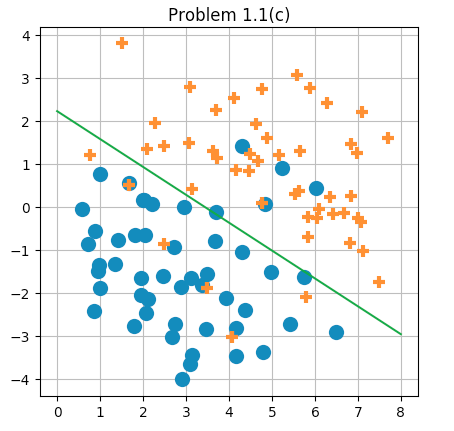
\includegraphics{images/pr1_1c.png}
\caption{The data points given for problem 1.1 along with the decision
boundary learned by logistic regression as executed by Newton's method.}
\end{figure}

\subsection{Poisson regression and the exponential
family}\label{poisson-regression-and-the-exponential-family}

\subsubsection{Part (a)}\label{part-a-1}

Write the Poisson distribution as an exponential family:

\[p(y;\eta) = b(y)\exp\big(\eta^T T(y) - a(\eta)\big),\]

where

\[p(y;\lambda) = \frac{e^{-\lambda}\lambda^y}{y!}.\]

This can be done via

\[\begin{array}{rcl}
\eta & = & \log(\lambda), \\
a(\eta) & = & e^\eta = \lambda, \\
b(y) & = & 1/y!, \text{ and} \\
T(y) & = & y.
\end{array}\]

\subsubsection{Part (b)}\label{part-b-1}

As is usual with generalized linear models, we'll let \(\eta = \th^Tx.\)
The canonical response function is then given by

\[g(\eta) = E[y;\eta] = \lambda = e^\eta = e^{\th^Tx}.\]

\subsubsection{Part (c)}\label{part-c-1}

Based on the last part, I'll define the hypothesis function \(h\) via
\(h(x) = e^{\th^Tx}.\)

For a single data point \((x, y),\) let \(\ell(\th) = \log(p(y|x)) =\)
\(\log(\frac{1}{y!}) + (y\th^T x-e^{\th^Tx}).\) Then

\[\frac{\partial}{\partial\th_j}\ell(\th) = yx_j - x_je^{\th^Tx}
= x_j(y-e^{\th^Tx}).\]

So stochastic gradient ascent for a single point \((x, y)\) would use
the update rule

\[\th := \th + \alpha x(y - h(x)).\]

\subsubsection{Part (d)}\label{part-d}

In section 1.10 of my notes --- the section on generalized linear models
--- I derived the update rule:

\[\th := \th + \alpha\big(T(y)-a'(\th^Tx)\big)x.\]

The missing piece is to proof that \(h(x) = E[y] = a'(\eta),\) which
we'll do next. We'll work in the context of \(T(y)=y,\) as given by the
problem statement. Notice that, for any \(\eta,\)

\[\int p(y)dy = \int b(y)\exp(\eta^Ty - a(\eta))dy = 1.\]

Since this identity is true for all values of \(\eta,\) we can take
\(\frac{\partial}{\partial\eta}\) of it to arrive at the value 0:

\[\begin{array}{rcl}
 0 & = & \frac{\partial}{\partial\eta}\int p(y)dy \\
   & = & \int \frac{\partial}{\partial\eta} b(y)\exp(\eta^Ty - a(\eta))dy \\
   & = & \int b(y)(y - a'(\eta))\exp(\eta^Ty - a(\eta)) dy \\
   & = & \int y p(y)dy - a'(\eta)\int p(y)dy \\
   & = & E[y] - a'(\eta).
\end{array}\]

Thus we can conclude that \(E[y] = a'(\eta) = a'(\th^Tx),\) which
completes the solution.

\subsection{Gaussian discriminant
analysis}\label{gaussian-discriminant-analysis}

\subsubsection{Part (a)}\label{part-a-2}

This problem is to show that a two-class GDA solution effectively
provides a model that takes the form of a logistic function, similar to
logistic regression. This is something I already did in section 2.1 of
\href{http://tylerneylon.com/notes/cs229/cs229.html}{my notes}.

\subsubsection{Parts (b) and (c)}\label{parts-b-and-c}

These parts ask to derive the maximum likelihood estimates of \(\phi,\)
\(\mu_0,\) \(\mu_1,\) and \(\Sigma\) for GDA. Part (b) is a special case
of part (c), so I'll just do part (c).

\textbf{Some lemmas}

It will be useful to know a couple vector- and matrix-oriented calculus
facts which I'll briefly derive here.

First I'll show that, given column vectors \(a\) and \(b,\) and
symmetric matrix \(C,\)

\begin{equation}\nabla_b [ (a-b)^T C (a-b) ] = -2C(a-b).\label{eq:nabla_b}\end{equation}

We can derive this by looking at the \(k^\text{th}\) coordinate of the
gradient. Let \(x = (a-b)^T C (a-b).\) Then, using repeated index
summation notation,

\[\begin{array}{crcl}
& x & = & (a_i - b_i)c_{ij}(a_j-b_j) \\
\Rightarrow & [\nabla_b]_k x & = & -c_{kj}(a_j - b_j) - (a_i - b_i)c_{ik} \\
 & & = & -2C(a-b). \\
\end{array}\]

Next I'll show that

\begin{equation}\frac{\partial}{\partial C}(a-b)^T C (a-b) = (a-b)(a-b)^T.\label{eq:partial_C}\end{equation}

This follows since

\[(a-b)^T C (a-b) = (a_i - b_i) c_{ij} (a_j - b_j),\]

so that

\[\frac{\partial}{\partial c_{ij}} (a-b)^T C (a-b)
= (a_i - b_i)(a_j - b_j).\]

In other words, the \(ij^\text{th}\) entry of the matrix derivative is
exactly the \(ij^\text{th}\) entry of the matrix \((a-b)(a-b)^T.\)

Finally, I'll mention that, when a matrix \(A\) is invertibe,

\begin{equation}\frac{d}{dA} |A| = |A|\,A^{-T}.\label{eq:deriv_of_det}\end{equation}

This can be seen by considering that the \(ij^\text{th}\) entry of
\(A^{-1}\) can be written as

\begin{equation}(A^{-1})_{ij} = ((-1)^{i+j}M_{ji})/|A|,\label{eq:inv_eqn}\end{equation}

where \(M_{ij}\) denotes the determinant of the minor of \(A\) achieved
by removing the \(i^\text{th}\) row and \(j^\text{th}\) column. Next,
consider the expression for \(A\) as a sum of products
\(\sigma(\pi)\prod a_{i\pi(i)}\) over all permutations \(\pi:[n]\to[n]\)
where \(\sigma(\pi)\) is the sign of permutation \(\pi\)
(\href{https://en.wikipedia.org/wiki/Determinant\#n_.C3.97_n_matrices}{reference}).
Based on that definition of a determinant, it can be derived that

\[\frac{\partial}{\partial a_{ij}}|A| = (-1)^{i+j}M_{ij}.\]

Combine this last result with (\ref{eq:inv_eqn}) to arrive at
(\ref{eq:deriv_of_det}).

\textbf{The solution}

We're now ready to derive the equations for the GDA parameters based on
maximum likelihood estimation.

The log likelihood function is

\[\ell = \sum_i \log(p(x|y)) + \log(p(y)).\]

\(\phi\)

\newcommand{\pd}[1]{\frac{\partial}{\partial #1}}

In this section I'll start to use the notation \([\textsf{Pred}(x)]\)
for the indicator function of a boolean predicate \(\textsf{Pred}(x):\)

\[[\textsf{Pred}(x)] := \begin{cases}
1 & \text{if }\textsf{Pred}(x)\text{ is true, and} \\
0 & \text{otherwise.} \\
\end{cases}\]

This is the notation that Knuth uses, and I prefer it to Ng's notation
\(1\{\textsf{Pred}(x)\}.\)

Treating \(p(y)\) as \(\phi^y(1-\phi)^{1-y},\) set \(\pd{\phi}\) of
\(\ell\) to 0; the result is

\[\sum_i\pd\phi\big(y\log\phi + (1-y)\log(1-\phi)\big)
= \sum_i \frac{y}{\phi} - \frac{1-y}{1-\phi} = 0\]

\[\Rightarrow\quad \sum_i y(1-\phi) - (1-y)\phi = 0\]

\[\Rightarrow\quad m_1 - m_1\phi = m_0\phi,\]

where \(m_j = \sum_i [y\toi = j],\) and I'm treating the possible \(y\)
values as 0 or 1. Then

\[m_1 = \phi(m_0 + m_1) \;\Rightarrow\; \phi = \frac{m_1}{m},\]

using that \(m = m_0 + m_1.\)

\(\mu_j\)

\newcommand{\Sinv}{\Sigma^{-1}}

\[\pd{\mu_j}\ell = \pd{\mu_j}\sum_{y=j}-\frac{1}{2}(x-\mu_j)^T\Sinv(x-\mu_j)\]

We can use (\ref{eq:nabla_b}) to see that this is the same as

\[\sum_{y=j} \Sinv(x-\mu_j).\]

Setting \(\pd{\mu_j}\ell = 0,\) and noticing that \(\Sinv\) must be
nonsingular as it's an inverse, we get

\[\sum_{y=j} x = \sum_{y=j} \mu_j,\]

resulting in

\[
\sum_{y=j} x = m_j \mu_j \quad \Rightarrow \quad
\mu_j = \frac{1}{m_j}\sum_{y=j}x
.\]

\(\Sigma\)

To get an equation for \(\Sigma,\) we'll actually maximize \(\ell\) with
respect to its inverse \(\Sinv.\) This works because there is a
bijection between all possible values of \(\Sinv\) and of \(\Sigma\)
under the constraint that \(\Sigma\) is invertible, which is required
for GDA to make sense. Thus the value of \(\Sinv\) which maximizes
\(\ell\) uniquely identifies the value of \(\Sigma\) which maximizes
\(\ell.\)

\[\pd{\Sinv}\ell = \sum_i\pd\Sinv\left(C + \frac{1}{2}\log |\Sinv| -
\frac{1}{2}(x-\mu_y)^T\Sinv(x-\mu_y)\right).\]

Use (\ref{eq:partial_C}) to see that this is the same as

\[\sum_i \frac{|\Sinv|\Sigma^T}{|\Sinv|} - \frac{1}{2}(x-\mu_y)(x-\mu_y)^T.\]

Set this value to 0 to arrive at

\[\sum_i \Sigma^T = \sum_i (x-\mu_y)(x-\mu_y)^T
\quad\Rightarrow\quad
\Sigma^T = \frac{1}{m}\sum_i (x-\mu_y)(x-\mu_y)^T.\]

Since the expression on the right must give a symmetric matrix, this
same expression also gives the value for \(\Sigma\) itself.

\subsection{Linear invariance of optimization
algorithms}\label{linear-invariance-of-optimization-algorithms}

\subsubsection{Part (a)}\label{part-a-3}

This problem is to show that Newton's method is invariant to linear
reparametrizations.

Specifically, suppose \(x^{(0)} = z^{(0)} = 0,\) that matrix \(A\) is
invertible, and that \(g(z) = f(Az).\) Our goal is to show that if the
sequence \(x^{(1)}, x^{(2)}, \ldots\) results from Newton's method
applied to \(f\), then the corresponding sequence
\(z^{(1)}, z^{(2)}, \ldots\) resulting from Newton's method applied to
\(g\) obeys the equation \(x^{(i)} = Az^{(i)}\) for all \(i,\) so that
the two versions of Newton's method are in a sense doing the exact same
work. We'll think of \(f\) consistently as a function of \(x,\) and
\(g\) as a function of \(z.\)

\newcommand{\pdd}[2]{\frac{\partial #1}{\partial #2}}

Start with

\[\big[\nabla_z g\big]_i = \pdd{f}{z_i} = \pdd{f}{x_j}\pdd{x_j}{z_i}
= \pdd{f}{x_j}a_{ji},\]

from which it follows that

\[\nabla g = A^T\nabla f.\]

Next, introduce the variables \(H\) as the Hessian of \(f,\) and \(P\)
as the Hessian of \(g.\) Then

\[
\begin{aligned}
p_{ij} & = \pd{z_i}\pdd{f}{z_j} = \pd{z_i}\left(\pdd{f}{x_k}a_{kj}\right)
= \left(\pd{z_i}\pdd{f}{x_k}\right)a_{kj} \\
& = \left(\pd{x_\ell}\pdd{x_\ell}{z_i}\pdd{f}{x_k}\right)a_{kj}
= \left(a_{\ell i}\frac{\partial^2f}{\partial x_\ell\partial x_k}\right)a_{kj}
= a_{\ell i}h_{\ell k}a_{kj}.
\end{aligned}
\]

We can summarize this as

\[P = A^T H A.\]

Newton's method in this context can be expressed by the two equations

\[\begin{aligned}
x^{(i+1)} & = x^{(i)} - H^{-1}(x^{(i)}) \nabla f(x^{(i)}), \text{ and} \\
z^{(i+1)} & = z^{(i)} - P^{-1}(z^{(i)}) \nabla g(z^{(i)}) \\
          & = z^{(i)} - (A^THA)^{-1}(x^{(i)}) A^T\nabla f(x^{(i)}). \\
\end{aligned}\]

We'll show by induction on \(i\) that \(x^{(i)} = Az^{(i)}\) for all
\(i.\) The base case for \(i=0\) is true by definition. For the
inductive step, assume that \(x^{(i)} = Az^{(i)},\) and use the above
equations to see that

\[\begin{aligned}
Az^{(i+1)} & = Az^{(i)} - AA^{-1}H(x^{(i)})A^{-T}A^T\nabla f(x^{(i)}) \\
           & = x^{(i)} - H(x^{(i)}) \nabla f(x^{(i)}) \\
           & = x^{(i+1)},
\end{aligned}\]

which completes this part of the problem.

\subsubsection{Part (b)}\label{part-b-2}

Gradient descent is not invariant to linear reparametrizations. The
update equation for \(f\) is

\[x^{(i+1)} = x^{(i)} - \alpha\nabla f,\]

and for \(g\) is

\[z^{(i+1)} = z^{(i)} - \alpha\nabla g = z^{(i)} - \alpha A^T\nabla f.\]

In order for \(Az^{(i+1)} = x^{(i+1)},\) we would need

\[A(z^{(i)} - \alpha A^T\nabla f) = Az^{(i)} - A\alpha\nabla f
\quad\Leftrightarrow\quad
AA^T\nabla f = A\nabla f,\]

but this is only guaranteed when \(A\) is unitary.

\subsection{Regression for denoising quasar
spectra}\label{regression-for-denoising-quasar-spectra}

\subsubsection{Part (a)}\label{part-a-4}

\begin{enumerate}
\def\labelenumi{\roman{enumi}.}
\item
\end{enumerate}

\newcommand{\up}[1]{^\text{#1}}

Let the \(i\up{th}\) row of \(X\) be \(x\toi.\) Then
\((X\th)_i = \langle x\toi,\th\rangle\) and
\((X\th - y)_i = \langle x\toi, \th\rangle - y\toi.\)

Let the \(i\up{th}\) diagonal element of \(W\) be \(\frac{w\toi}{2}.\)
Then
\(((X\th-y)^T W)_i = \frac{w\toi}{2}(\langle x\toi,\th\rangle-y\toi\rangle)\)
so that

\[J(\th) = (X\th - y)^T W (X\th - y) =
  \sum_i \frac{w\toi}{2}(\langle x\toi,\th\rangle - y\toi)^2.\]

This gives us a nice way to express \(J(\th)\) in terms of matrices and
vectors, as the problem requested.

\begin{enumerate}
\def\labelenumi{\roman{enumi}.}
\setcounter{enumi}{1}
\item
\end{enumerate}

This problem is to explicitly solve for \(\nabla_\th J(\th) = 0\) for
the function \(J(\th)\) given in the last part.

I'll begin by defining the general notation

\[\langle a, b \rangle_W := a^T W b.\]

This is similar to a standard inner product when both \(a\) and \(b\)
are column vectors, but the notation still works when \(a\) or \(b\) are
matrices of appropriate dimensions.

Let's find some gradient formulas for
\(\nabla_\th \langle a, b\rangle_W\) in the case that \(a, b\) depend on
\(\th\) but \(W\) doesn't. It will be useful to keep in mind that

\[\langle a, b \rangle_W = a_i w_{ij} b_j.\]

Then

\[\pd{\th_k}(a_i w_{ij} b_j) = a'_i w_{ij} b_j + a_i w_{ij} b'_j,\]

where \(x'\) denotes \(\pdd{x}{\th_k}.\)

Define the matrix \(A'\) so that it has \(k\up{th}\) column
\(\pd{\th_k} a,\) and similarly for \(B'\) from \(b.\) Then

\[\pd{\th_k}\langle a, b\rangle_W
  = \langle \pdd{a}{\th_k}, b \rangle_W
  + \langle a, \pdd{b}{\th_k} \rangle_W,\]

which we can summarize as

\[\nabla_\th \langle a, b\rangle_W = \langle A',b \rangle_W
                                   + \langle a,B' \rangle_W^T.\]

In the special case that \(W\) is symmetric, we also have

\[\begin{aligned}
\nabla_\th \langle z, z \rangle_W
  & = \langle Z', z\rangle_W + \langle z, Z' \rangle_W^T \\
  & = \langle Z', z\rangle_W + (z^T W Z')^T \\
  & = \langle Z', z\rangle_W + Z'^T W z \\
  & = 2 \langle Z', z\rangle_W, \\
\end{aligned}\]

which can be summarized as

\[\nabla_\th \langle z, z \rangle_W = 2\langle Z', z\rangle_W.\]

To get back to the actual problem, notice that, by letting
\(z = X\th - y,\) we can write \(J = \langle z, z \rangle_W.\)

Then

\[\begin{aligned}
\nabla J & = 2\langle Z', z\rangle_W \\
& = 2 Z'^T W z \\
& = 2 X^T W z \\
& = 2 X^T W (X \th - y) = 0 \\
\Rightarrow \; X^T W X \th & = X^T W y \\
\Rightarrow \; \th & = (X^T W X)^{-1} X^T W y
 = (\langle X, X\rangle_W)^{-1} \langle X, y \rangle_W, \\
\end{aligned}\]

which is the closed-form expression the problem asked for.

\begin{enumerate}
\def\labelenumi{\roman{enumi}.}
\setcounter{enumi}{2}
\item
\end{enumerate}

In this problem, we suppose that

\[(y\toi \mid x\toi) \sim \mathcal N(\th^T x\toi, \sigma\toi).\]

Our goal is to show that maximizing the log likelihood in this scenario
is the same as an application of weighted linear regression as seen in
the previous two parts.

Begin by writing that

\[\begin{aligned}
\ell(\th) & = \sum_i \log\left(c_i \exp\left(
    -\frac{(y\toi - \th^T x\toi)^2}{2(\sigma\toi)^2}\right)\right) \\
  & = \sum_i \log(c_i) - \frac{(y\toi - \th^T x\toi)^2}{2(\sigma\toi)^2},
\end{aligned}\]

where \(c_i\) is a value independent of \(\th,\) so that we may safely
ignore it when taking \(\nabla_\th.\)

From this point on I won't write the \(i\) index on variables. I hope
it's clear from context. Then

\[\nabla_\th \ell = \sum_i \frac{2(y - \th^T x)x}{2\sigma^2},\]

so that \(\nabla\ell = 0\) when

\[\sum_i \frac{1}{\sigma^2}(y - \th^T x)x = 0.\]

Let the \(k\up{th}\) diagonal element of \(W\) be
\(1/(\sigma^{(k)})^2,\) and define matrix \(X\) so that its \(i\up{th}\)
row is \(x\toi.\) Also let \(\vec y\) denote the column vector with
\(i\up{th}\) coordinate \(y\toi.\) Then

\[\sum_i \frac{1}{\sigma^2}(y - \th^T x)x = X^T W (\vec y - X\th).\]

This can be confirmed by seeing that the column vector
\(m = W(\vec y - X\th)\) has \(i\up{th}\) coordinate
\(\frac{1}{(\sigma\toi)^2}(y\toi - \th^T x\toi),\) and seeing the
product \(X^T m\) as \(\sum_i x\toi m_i.\)

But this last expression matches what we found in part \emph{ii} of this
problem, showing that solving this maximum likelihood estimate is
effectively the same as solving a weighted linear regression problem.

\subsubsection{Part (b)}\label{part-b-3}

i

I interpret this problem as applying linear regression to the first row
of the given data file as a function of the wavelengths. This is the
Python code I used:

\begin{verbatim}
#!/usr/bin/env python
"""Problem 1_5b_i.py

Graph the first row of data and a linear regression for
this data.
"""

import matplotlib.pyplot as plt
import numpy as np
import numpy.linalg as la


# Load the data.
all_data = np.loadtxt('quasar_train.csv', delimiter=',')
lambdas  = all_data[0, :]
data     = all_data[1:, :]
row1     = data[0, :]

# Run least squares.
A    = np.vstack((lambdas, np.ones(len(lambdas)))).T
m, c = la.lstsq(A, row1)[0]

# Plot the data and line.
plt.plot(lambdas, row1, 'o', label='spectra data',
    markersize=2)
plt.plot(lambdas, m * lambdas + c, 'r', label='fitted line')
plt.title('Problem 1.5(b)i')
plt.legend()
plt.show()
\end{verbatim}

The code generated this image:

\begin{figure}[htbp]
\centering
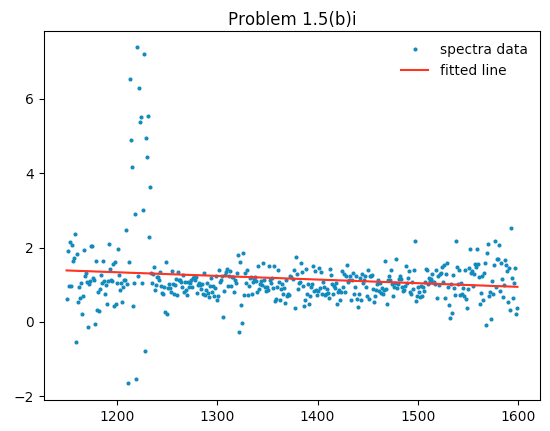
\includegraphics{images/pr1_5bi.png}
\caption{The first row of quasar spectra data plotted against
wavelengths along with the line of best fit.}
\end{figure}

The line found had a slope of -0.000981122145459 with an intercept value
of 2.5133990556. In other words, the spectra value \(v\) is approximated
via the equation

\[v = 2.5134 - 9.8112\mathrm{e}{-4} \, \lambda,\]

where \(\lambda\) is the wavelength.

ii

Here is the code:

\begin{verbatim}
#!/usr/bin/env python
"""Problem 1_5b_ii.py

Graph the first row of data along with a locally weighted
linear regression.
"""

import matplotlib.pyplot as plt
import numpy as np
import numpy.linalg as la


# A function to solve locally weighted linear regression for
# given matrices X and W.
def lwlr_theta(X, W, y):
  A = X.T.dot(W)
  B = A.dot(X)
  return la.inv(B).dot(A).dot(y)

def lwlr_at_pt(all_x, y, query_x):
  X     = np.vstack((np.ones(len(all_x)), all_x)).T
  x     = query_x
  tau   = 5
  denom = 2.0 * tau ** 2
  w     = np.exp([-(x - xi) ** 2/denom for xi in all_x])
  W     = np.diag(w)
  theta = lwlr_theta(X, W, y)
  return theta[0] + theta[1] * query_x

def main():
  # Load the data.
  all_data = np.loadtxt('quasar_train.csv', delimiter=',')
  lambdas  = all_data[0, :]
  data     = all_data[1:, :]
  row1     = data[0, :]

  # Compute the LWLR curve at each lambda.
  curve = [lwlr_at_pt(lambdas, row1, x) for x in lambdas]

  # Plot the data and line.
  plt.plot(lambdas, row1, 'o', label='spectra data',
      markersize=2)
  plt.plot(lambdas, curve, 'r', label='LWLR curve')
  plt.title('Problem 1.5(b)ii')
  plt.legend()
  plt.show()

if __name__ == '__main__': main()
\end{verbatim}

Here is the graph generated:

\begin{figure}[htbp]
\centering
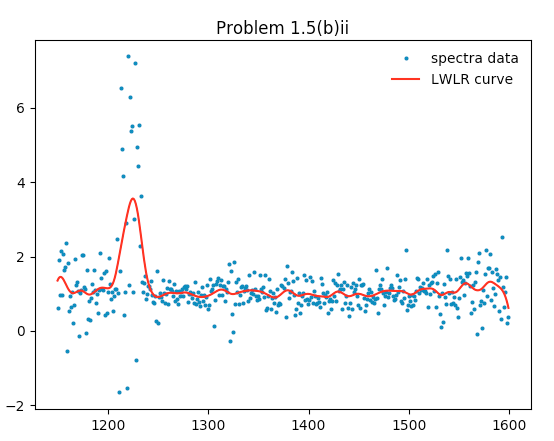
\includegraphics{images/pr1_5bii.png}
\caption{The first row of quasar spectra data plotted against
wavelengths along with the curve resulting from a locally weighted
linear regression with \(\tau = 5.\)}
\end{figure}

\end{document}
